\documentclass[12pt,a4paper]{article}
\usepackage[utf8]{inputenc}
\usepackage{listings}
\usepackage{subfigure}
\usepackage{graphicx}
\usepackage{color}
\usepackage{xcolor}
\usepackage{caption}
\usepackage[backend=bibtex, style=numeric, bibstyle=ieee]{biblatex}
\bibliography{report}
\usepackage{hyperref}
\usepackage{multicol}
\usepackage{longtable}
\usepackage{amsmath}
\usepackage{setspace}
\usepackage[margin=1in]{geometry}
\doublespacing
%\usepackage{tikz}
%\usetikzlibrary{arrows,automata}
%
%\definecolor{mygreen}{rgb}{0,0.6,0}
%\definecolor{mygray}{rgb}{0.5,0.5,0.5}
%\definecolor{mymauve}{rgb}{0.58,0,0.82}

\usepackage{caption}

\author{Lingyan Zhou \and Jianhong Zhu}
\date{\today}
\title{Tipping behavior analysis with Hadoop}
\begin{document}
\maketitle

\begin{abstract}
  Taxis are a reliable data source of public transportation and people's tipping behavior. However, the huge amount of data generated by every taxi poses a problem to effectively discover hidden facts from it using conventional computing techniques. Thus we implemented several command-line applications using the Hadoop MapReduce. We incorporated common MapReduce patterns and some special computational techniques that can yield results in one MapReduce job. Our implementations can process five Giga-bytes of compressed taxi trip data in two minutes on average.
\end{abstract}

\newpage

\tableofcontents
\newpage

\section{Introduction}
With the recent advancement in big data technologies, more and more industries now base their businesses and profits on data-driven decision making. For metropolis like New York city, the data generated from its primary mode of transportation, taxi, is a valuable indicator for urban planning, public transportation scheduling and people's daily commuting arrangement. More specifically, taxi companies can analyze the data and direct drivers to more profitable customers, time and areas in greatest demand for fast transit to compete with fast growing star-up companies like Uber and Lyft.

In an attempt to improve the accessibility, transparency, and accountability, the New York Taxi and Limousine Commission has released millions of taxi trip records from 2011\cite{nyctlcwebsite}. The whole data set contains 540 million records per year. Many researchers have used the taxi trip data set for various purposes. To help others build an intuitive understanding of huge data set, the Chris Whong built a web-based visualization tool to animate every taxi trip on a map\cite{nyctaxyvisualwebsite}. Whong's application inspired developers at ImageWork, they associated flight trips with taxi trips from two major airports and also built a similar visualization tool\cite{flighttaxiwebsite}. Similar applications include \cite{hubcabwebsite}, a multi-resolution traffic density viewer. Apart from data visualization, there were also attempts to analyze the data statistically. Ryan Hafen did an initial analysis using R using a sample set, which showed basic statistics of trip distances, tip amount and etc\cite{hafenwebsite}. Hafen's work also revealed the relationship between pickup counts and locations\cite{hafenwebsite}. This dataset also attracted academic researches. In \cite{andrewj}, Andrew James discussed in details about sanitizing the data set, made comprehensive plots and proposed a ride sharing framework based on pixelized taxi density map. 

In this article, we aimed to discover some interesting tipping patterns by examining the June to October, 2013 New York taxi trip data set. In this data set, there are 54 million trip records. Each trip has the following fields: medallion number, hack license number, pickup date and time, drop-off date and time, passenger count, trip duration (in seconds), trip distance, pickup latitude and longitude, drop-off latitude and longitude, tip and fare amount and etc. However, the fare and trip information of every record are separated in two different files.A record description was distributed along with the data\cite{nyctaxidatadict}.

To effectively compute the statistics, we used Hadoop. Hadoop is a Java implementation of Google's MapReduce framework, which simplifies distributed computing by separating computation in mapping and reducing phases. However, the framework also requires special computational techniques to achieve its maximum performance. For example, each mapper only receives a part of a large data set and there is no way to pass messages between mappers. In this article, we present our attempt to use Hadoop to process and analyze the taxi trip data. We implemented efficient algorithms to make calculation of standard deviations, auto-correlations and etc. finish in one MapReduce job.

\section{Methods}
In this section, we first preprocessed the data to make it more Hadop-friendly. Then we took a 1\% sample of the original data and visualized it using simple matrix plot. This step helped us gain more insight to the data. Next, we detected outliers and erroneous data based on \cite{andrewj}. We implemented several Java command-line application on Hadoop to do the following calculation\cite{projrepo}. In order to determine the quality of the data set, we calculated summary statistics of most fields without removing outliers. Then, with outliers filtered out, we uncovered relationships and dependencies between fields. With the temporal and spacial information in the data set, we found the seasonality of tip amount using autocorrelation, pixelized the average tip amount in regions. Most frequent tip amount and tip ration was also discovered by data binning. Finally, we built a K-nearest-neighbor tip predictor. 

\subsection{Data Preprocessing}
The simplification of MapReduce framework brought everyday programmers to distributed computing. However, the simplified computation model also restricted its application. One disadvantage of it is to perform join operations of two files. Note that the data we got was separated in two files that needs joining. We wrote a Python script to combine the files line by line and then produce a single compressed file. For easy uploading the data onto the Hadoop clusters, we separated the file into eighteen 200MB chunks. 

Note that according to \cite{hdbestpract}, Hadoop splits files into blocks and when running MapReduce jobs, each block will spawn a mapper task. Because the start-up of a mapper takes time and there are also management overhead with each mapper, \cite{hdbestpract} suggests that the file size should not be too small compared with the block size. In our setup, we used 128MB as the block size. So each 200MB chunk will need 2 mappers, with slightly unbalanced load.

We did not perform data cleansing in this phase. Filtering obvious erroneous records was done on the MapReduce framework to demonstrate the use of filtering pattern (see Section \ref{sec:filtering}).

\subsection{Visualizing Sample Data}
\label{sec:initialexpl}
In order to gain more insight to the data, we worked on a smaller subset of the data, with 0.1\% sample size. The sample was selected at random without replacement. Like in \cite{hafenwebsite}, we performed initial statistical and visual investigation with R. Part of the statistical summary is shown in Table \ref{tab:rsummary}.

\begin{table}[h]
  \centering
  \caption{Summary on fare and tip of 1\% sample}
    \label{tab:rsummary}
    \begin{tabular}{|r|c|c|c|} \hline
      \multicolumn{2}{|c|}{fare amount}   & \multicolumn{2}{|c|}{tip amount} \\ \hline
      Min.   & -5.00  &  Min.   & 0.000   \\ \hline
      1st Qu.&  6.50  &  1st Qu.& 0.000   \\ \hline
      Median &  9.50  &  Median & 1.000   \\ \hline
      Mean   & 12.53  &  Mean   & 1.366   \\ \hline
      3rd Qu.& 14.50  &  3rd Qu.& 2.000   \\ \hline
      Max.   &229.00  &  Max.   &76.500 \\ \hline
    \end{tabular}
  \end{table}

  The tabulated summary indicated that 1) the data quality is good in terms of the number of  outliers, 2) the distribution of the variables in terms of inter-quartile ranges. In Section \ref{sec:assortedsummary}, we also summarized on the unsampled data set with Hadoop.

  Visually, we used R's matrix plot to visualize relationships between variables (see Figure \ref{fig:rmatrixplot}). 

  \begin{figure}[h]
    \centering
    \caption{Matrix plot of trip duration, distance, fare and tip}
    \label{fig:rmatrixplot}
    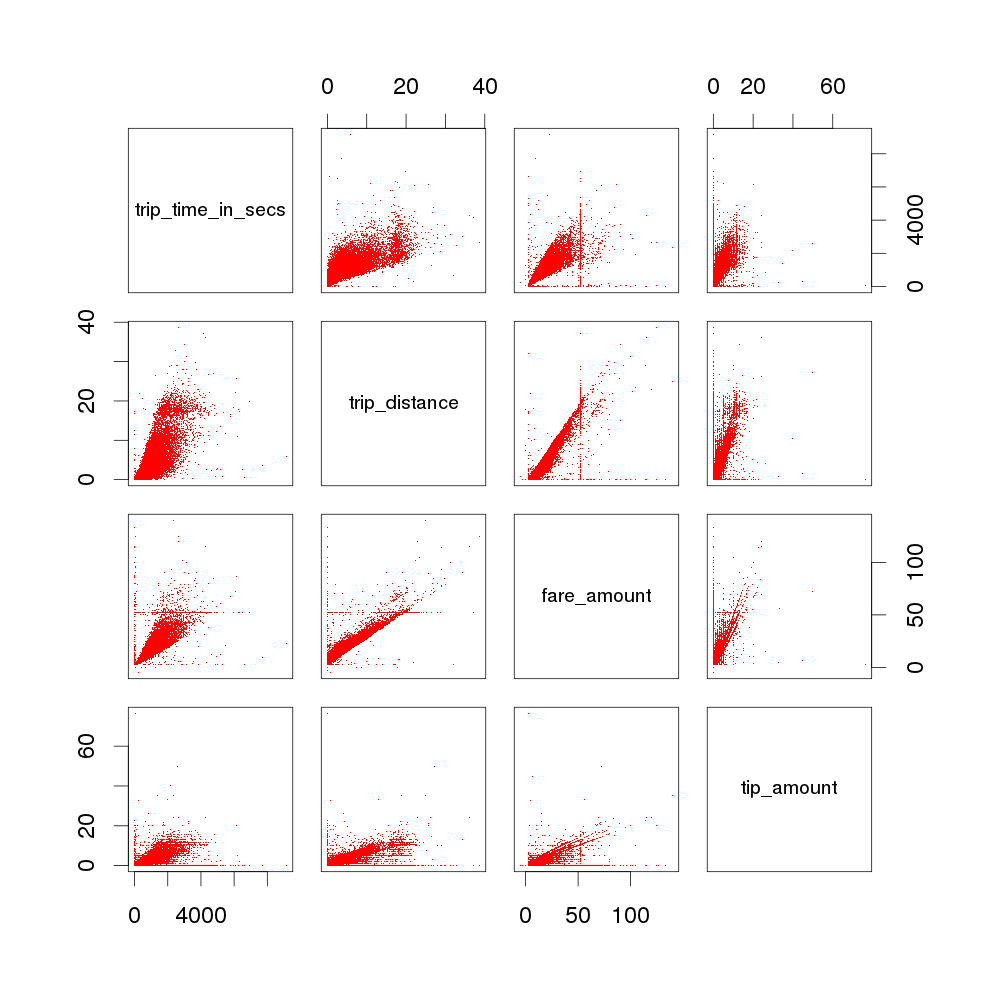
\includegraphics[scale=0.3]{plot/matrixplot}
  \end{figure}

  The plot shows linear relationships between each pair of the four variables, trip duration, distance, fare and tip. Beyond the obvious linear relationships, we also discovered some strips in the tip versus fare plot. We suspected that these trips indicated tipping norms and we intended to verify it using the unsampled data set (see Section \ref{sec:freqamounts}).

  \subsection{Data Filtering}
  \label{sec:filtering}
  Any ``big data'' data set has some erroneous records and the taxi data set was not an exception. Such errors might result from broken GPS devices, inaccurate driver-entered data (like the passenger count), and human errors in data compilation process. We identified such invalid records according to \cite{nyctaxidatadict}, \cite{andrewj}, and \cite{hafenwebsite}. For example, tips that exceeded 200 dollars were considered as invalid. For the geographical information like latitude and longitude, we restricted them inside longitude (-74.05, -73.70) and latitude (40.60, 40.85). Note that they were not the actual city boundary, but they suffice for our analysis. 

  In our implementation, the filtering happened in two phases. The first filter was inside the record reader object, marking invalid fields and records as ``NA'' values. As it was in the record reader, the filter was mandatory. The second filter was implemented as a mapper. It removed any record with an "NA" field. This filter was used in all our analysis except in Section \ref{sec:assortedsummary}.

  \subsection{Assorted Statistical Summaries}
  \label{sec:assortedsummary}
  Moving from sample data to the real data, we used Hadoop to facilitate processing speed. The first thing is to reproduce a similar summary report without sampling. We employed the Hadoop summarization pattern. Taking mean value calculation for example, in the mappers, we needed to keep track of per-mapper summation and record number, and in the singleton reducer, we combined the partial results and thus get the global mean value. 

  Unlike the summary report in R, we used standard deviation as a measure of distribution. It is commonly used to measure the spread of a variable. The definitive equation is in Equation \ref{eq:stddev}.
  \begin{equation}
    \label{eq:stddev}
    var(X) = \sqrt{E(X-E(X))}
  \end{equation}
  Using this equation, we need to separate the calculation into two MapReduce jobs, the first to calculate the mean, the second to calculate the standard deviation. As this calculation is not complicated and the process is obviously IO-bond, we intended to save the IO time by squeezing the calculation in one MapReduce job. We used the alternative standard deviation formula as shown in \ref{eq:stddev2}. 
  \begin{equation}
    \label{eq:stddev2}
    var(X) = \sqrt{E(X^2)-E(X)^2}
  \end{equation}
  Adopting this formula, our program kept track of the summation, the summation of squared values, and the total number of records in each mapper. In this way the standard deviation can be calculated in one pass. The result is shown in Table \ref{tab:numsum}.
  \begin{table}[h]
    \centering
    \caption{Numerical variable summary}
    \label{tab:numsum}
    \begin{tabular}{|l|c|c|c|c|c|} \hline
      column	&	min	&	max	&	average	&	std dev	&	missing percent \\ \hline
      trip distance	&	0.00	&	500.00	&	2.96	&	3.49	&	0.0000 \\ \hline
      trip time in secs	&	0.00	&	17820.00	&	767.98	&	575.94	&	0.0001 \\ \hline
      passenger count	&	0.00	&	8.00	&	1.70	&	1.37	&	0.0000 \\ \hline
      dropoff latitude	&	40.60	&	40.85	&	40.75	&	0.03	&	0.0201 \\ \hline
      dropoff longitude	&	-74.05	&	-73.70	&	-73.97	&	0.03	&	0.0168 \\ \hline
      mta tax	&	0.00	&	0.50	&	0.50	&	0.03	&	0.0001 \\ \hline
      fare amount	&	0.00	&	500.00	&	12.56	&	10.27	&	0.0001 \\ \hline
      tip amount	&	0.00	&	200.00	&	1.38	&	2.21	&	0.0000 \\ \hline
      surcharge	&	0.00	&	1.50	&	0.32	&	0.36	&	0.0000 \\ \hline
      pickup longitude	&	-74.05	&	-73.70	&	-73.98	&	0.04	&	0.0141 \\ \hline
      pickup latitude	&	40.60	&	40.85	&	40.75	&	0.02	&	0.0143 \\ \hline
      tolls amount	&	0.00	&	151.99	&	0.26	&	1.24	&	0.0000 \\ \hline
      total amount	&	0.00	&	699.96	&	15.02	&	12.32	&	0.0001 \\ \hline
    \end{tabular}
  \end{table}

  The result was consistent with our initial exploration with R. For most people, taxi was a short-distance transportation method. The outliers in each field does not exceed 2\% of the records, indicating the reliability of the data. Note especially the total records was 54 million, but in this and some other calculations, we got 91 million. The reason is that we customized the input data format without paying attention to the unsplittable gzip format, resulting in 2 mappers reading some overlapped portions of the same file. As we write this article, the bug has been fixed, thanks to \cite{hadoopsource}.

  For categorical variables, we summarized the frequency of each level using Hadoop word count pattern. The result is shown in Figure \ref{fig:catsum}. The figure indicated that 1) the two venders had similar market shares; 2) people preferred to pay by credit card; 3) most trips were in downtown, followed by trips from and to JKF airport.

  \begin{figure}[h]
    \centering
    \caption{Categorical variable summary}
    \label{fig:catsum}
    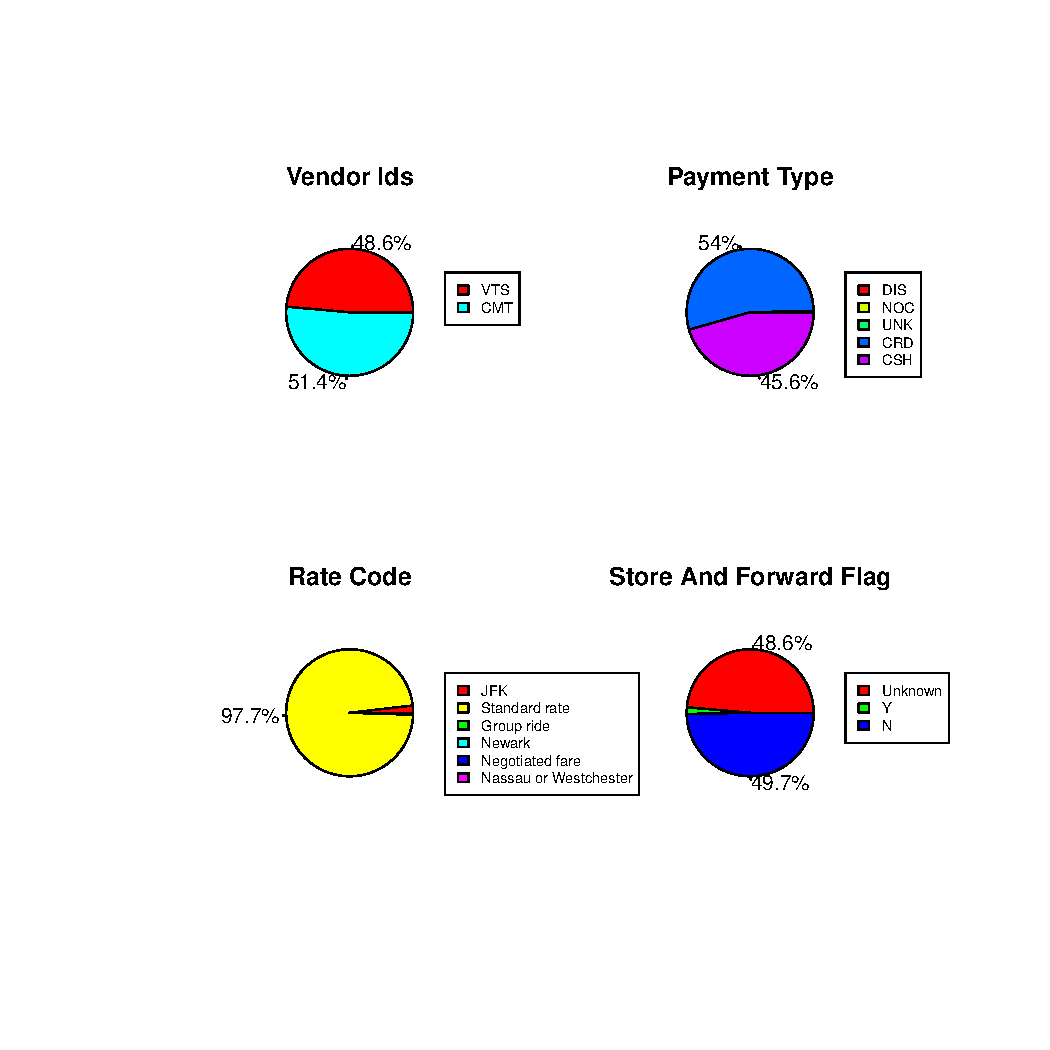
\includegraphics[scale=0.6]{plot/factor_summary}
  \end{figure}

  \subsection{Correlations and Dependency}
  Based on our initial exploration in Section \ref{sec:initialexpl}, we wanted to confirm that some variables have linear correlations. For numerical variables, we used Pearson correlation coefficients. It is defined in Equation \ref{eq:pearsoncorr}. Again, computation was less demanding than IO. So it was sensible to use an equivalent equation (as described in Equation \ref{eq:pearsoncorr2}) to fit the computation in one MapReduce job. 
  \begin{equation}
    \label{eq:pearsoncorr}
    \rho =\frac{E(x-\bar{x})(y-\bar{y})}{\sigma_x\sigma_y}
  \end{equation}
  \begin{equation}
    \label{eq:pearsoncorr2}
    \rho =\frac{E(x)E(y)-E(xy)}{\sqrt{E(x^2)-E(x)^2}\sqrt{E(y^2)-E(y)^2}}
  \end{equation}
  \begin{figure}[h]
    \centering
    \caption{Correlation matrix}
    \label{fig:corrmatrix}
    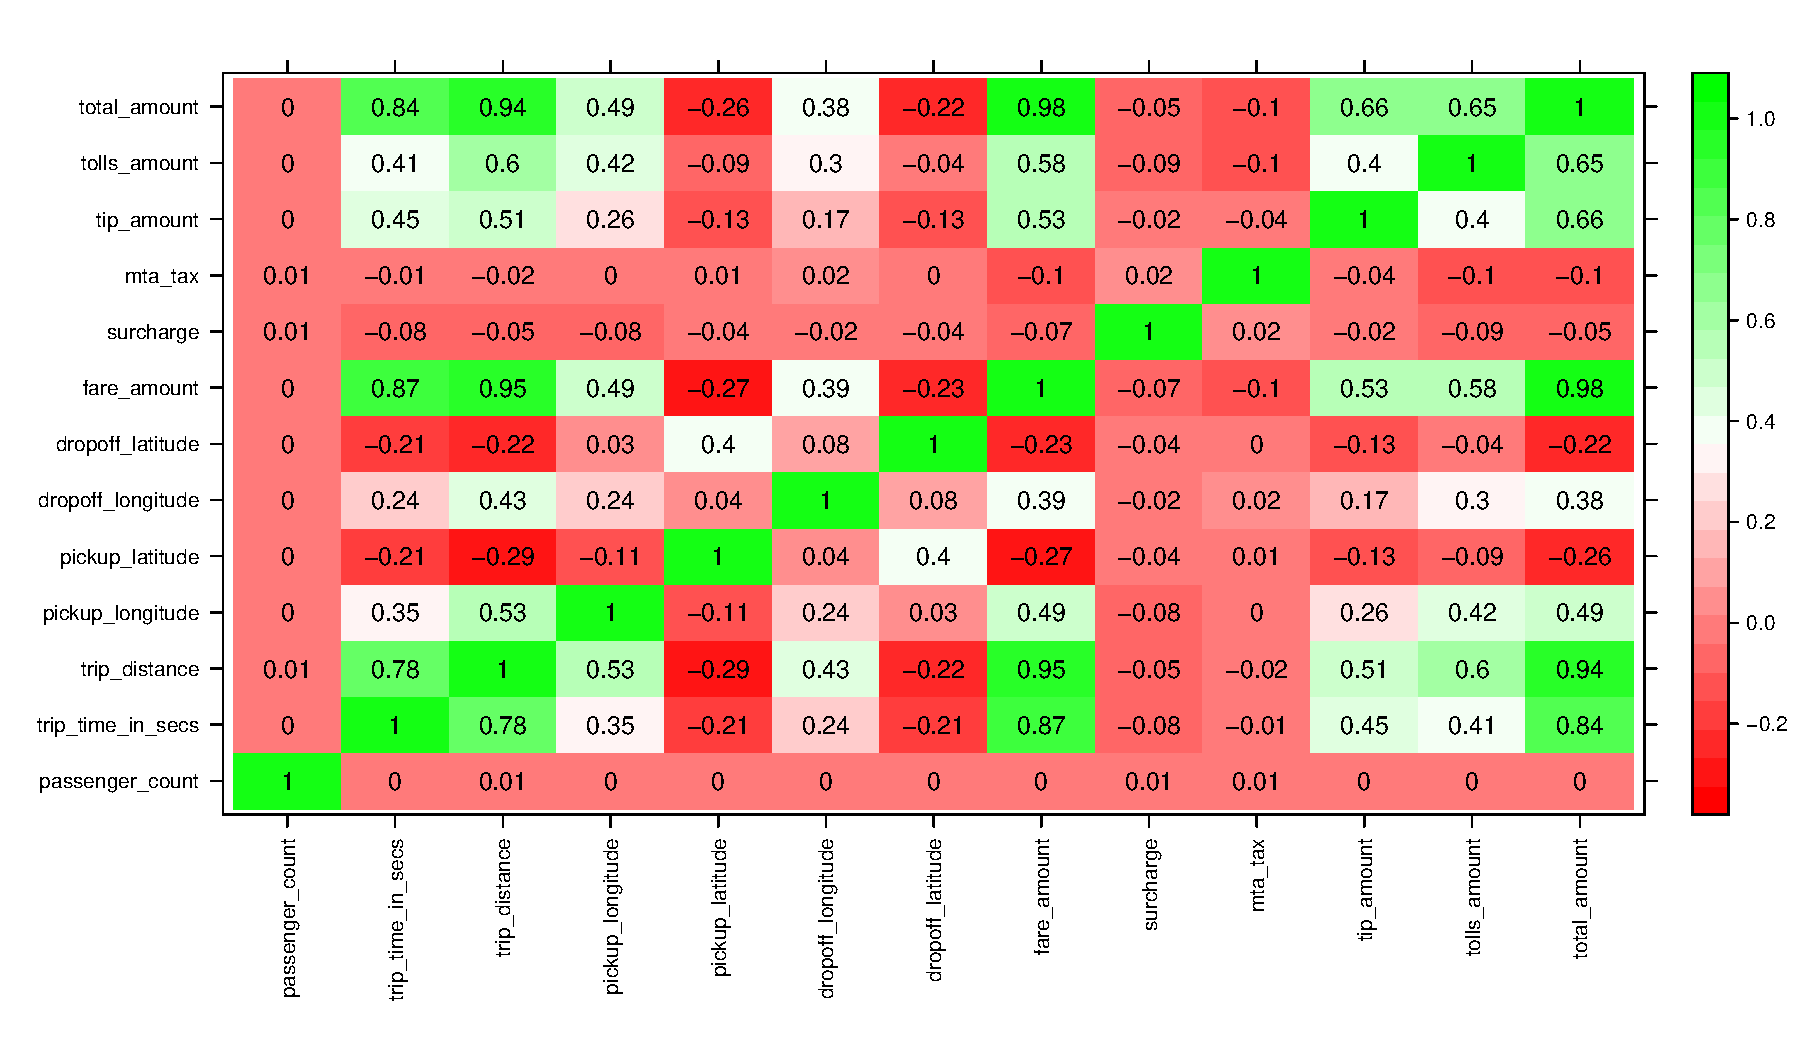
\includegraphics[scale=0.4]{plot/corrmatrix}
  \end{figure}
  The results shown in Figure \ref{fig:corrmatrix} indicates that trip fares were a possible primary factor that affected how people pay tips. Surprisingly, the correlation coefficient of tip and fare is not close to 1. This might be caused by not filtering out transactions with cash as its payment type, where tips were not recorded and were always 0.

  A typical statistical test of independence is called $\chi^2$ test. The calculation includes building up a contingency table, calculating the expected values and then get the sum of squared error\cite{chisqwebsite}. The resulting value is then compared with a table to determine dependence. In Hadoop, the challenge was to construct the contingency table. We used the structural pattern. The table was implemented as a data structure and each mapper used this structure as output. Then the reducer combined tables from mappers and calculated the $\chi^2$ value. The result is shown in Table \ref{tab:chisq}. All these value is greater than the 5\% confidence reference value. 
  \begin{table}[h]
    \center
    \caption{$\chi^2$ test of independence}
    \label{tab:chisq}
    \begin{tabular}{|c|c|}\hline
      vender id \& rate code	& 2.37E4 \\ \hline
      payment type \& rate code	& 7.64E5 \\ \hline
      store fwd flag \& rate code	& 3.45E4 \\ \hline
      payment type \& store fwd flag	& 3.19E5 \\ \hline
      vender id \& payment type	& 3.15E5 \\ \hline
      vender id \& store fwd flag	& 8.9E7 \\ \hline
    \end{tabular}
  \end{table}

  \subsection{Interesting Tipping Behavior}
  \label{sec:freqamounts}
  \label{sec:freqratios}
  In the following analysis, we filtered out all records with payment type being cash, because no tip was recorded. We built histograms of tip amount, tip ratios, locations, and time. After building a histogram of time, We also analyzed the temporal pattern using autocorrelation. The reason to use histogram was the continuous nature of the ratios, time and locations. Hadoop binning pattern was used.

  The bin width for tip amount was 0.01 dollar. The bin width for ratio was 0.01 radius. The results are shown in Figure \ref{fig:tipamounthist} and \ref{fig:tipratiohist}. Clearly, people tended to tip at integer amount, followed by amount that was multiple of 0.5 and 0.25 dollar, and at 20\%, 10\%, and 15\%. Note that some gaps and peaks were caused by the inaccuracy of floating point values. However, the overall distribution was not affected.

  \begin{figure}[h]
    \centering
    \caption{Interesting Tipping Behaviors}
    \subfigure[Tip amount histogram]{
      \label{fig:tipamounthist}
      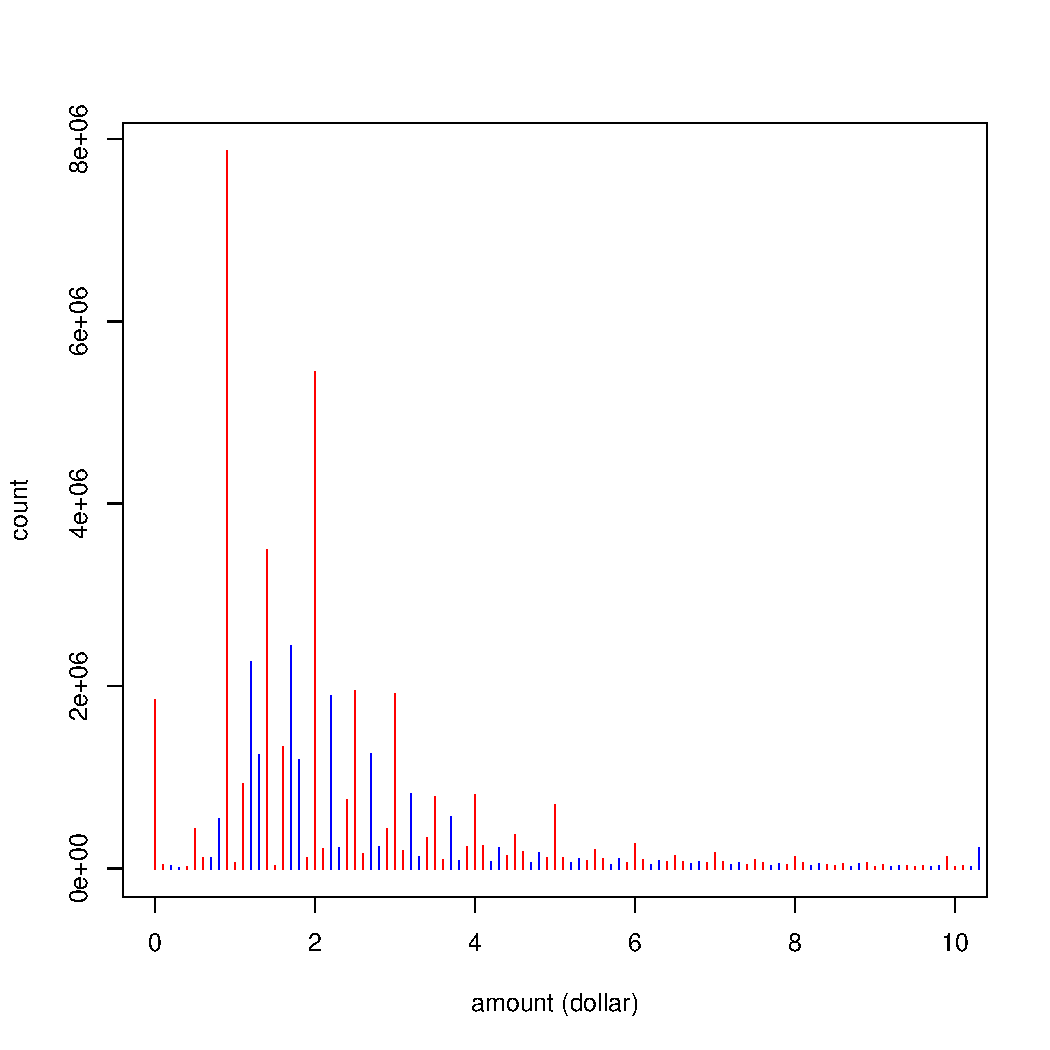
\includegraphics[scale=0.35]{plot/tipamounthist}
    }
    \subfigure[Histogram of tip ratio]{
      \label{fig:tipratiohist}
      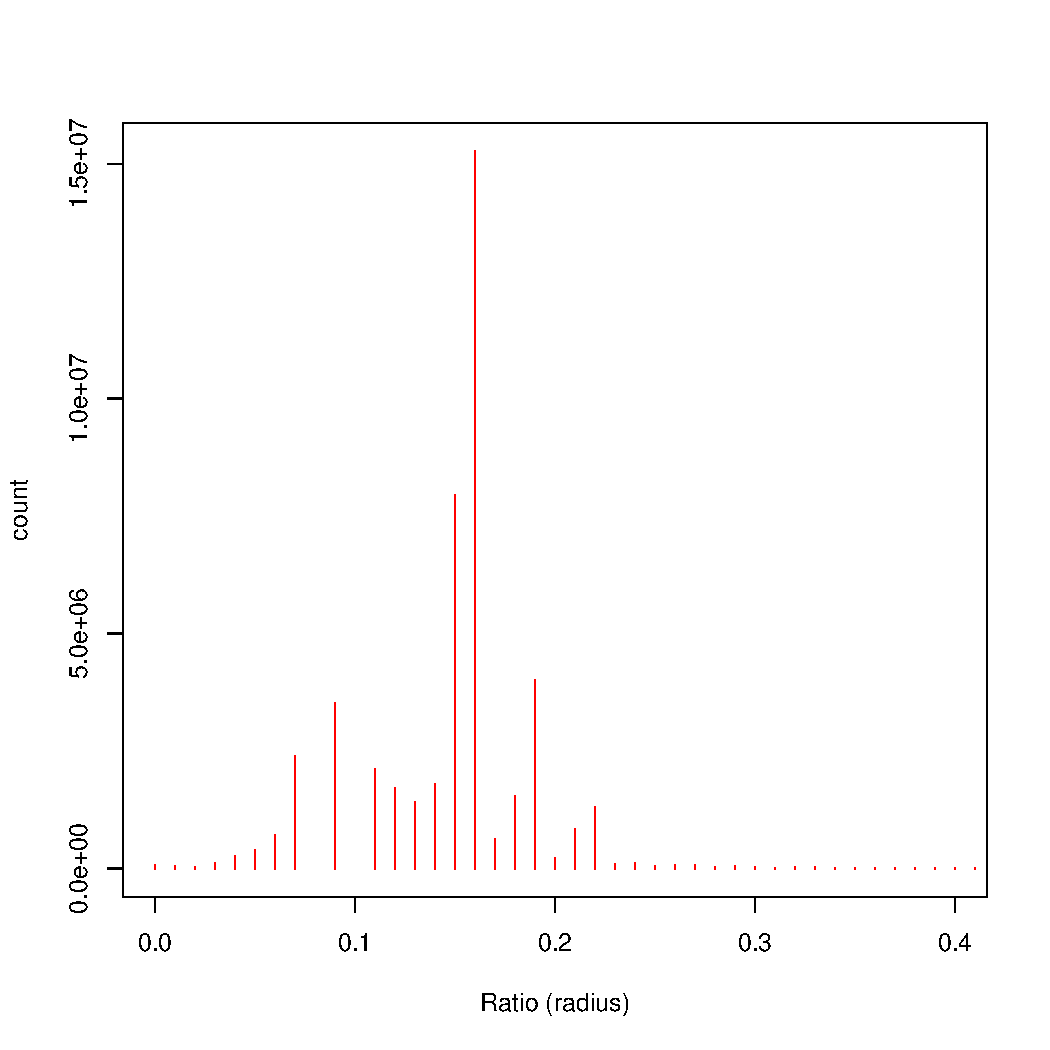
\includegraphics[scale=0.35]{plot/tipratiohist}
    }
  \end{figure}

  Average tips were binned according locations. The bin size was chosen so that the New York city was divided into 1000x1000 pixels. Hadoop Top-K pattern was used to select the top 100 locations with most average tips. The result is illustrated in Figure \ref{fig:toplatlog}. Highest average tips were concentrated around the downtown area and the JFK airport.
  \begin{figure}[h]
    \centering
    \caption{Location with most tip}
    \label{fig:toplatlog}
    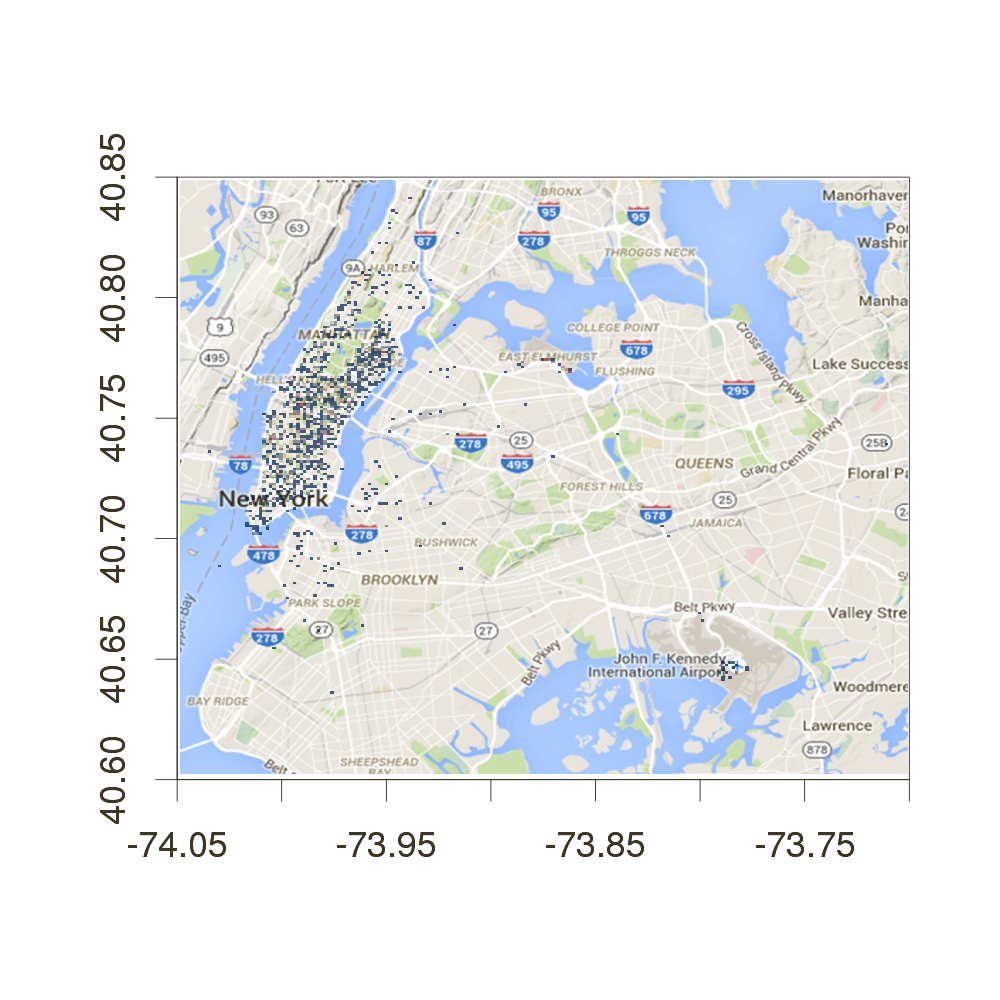
\includegraphics[scale=0.2]{plot/map}
  \end{figure}


  The trip data set contained pickup time. Thus we could use some common techniques in dealing with time series. A basic attribute is seasonality. To find seasonality, auto-correlation is commonly used. Its strict definition is described in Equation \ref{eq:autocorr}. We used a simpler definition (see Equation \ref{eq:autocorr2}) that was commonly used in signal processing areas.
  \begin{equation}
    \label{eq:autocorr}
    \rho_{xx}(\tau) =\frac{E(x_{t}-E(x))(x_{t+\tau}-E(x))}{\sigma_x^2}
  \end{equation}
  \begin{equation}
    \label{eq:autocorr2}
    \rho_{xx}(\tau) =\sum{x_{t}x_{t+\tau}}
  \end{equation}

  This task was separated into two MapReduce jobs. The first binned tip amounts into hours. The second did the calculation. Again, we used structural pattern so that a reducer could receive a variable and time delayed versions of itself. The results are shown in Figure \ref{fig:autocorr}.

  \begin{figure}[h!]
    \centering
    \caption{Seasonality of tipping behavior}
    \label{fig:autocorr}
    \subfigure[Autocorrelation of hourly tip sum]{
      \label{fig:tipsumautocorr}
      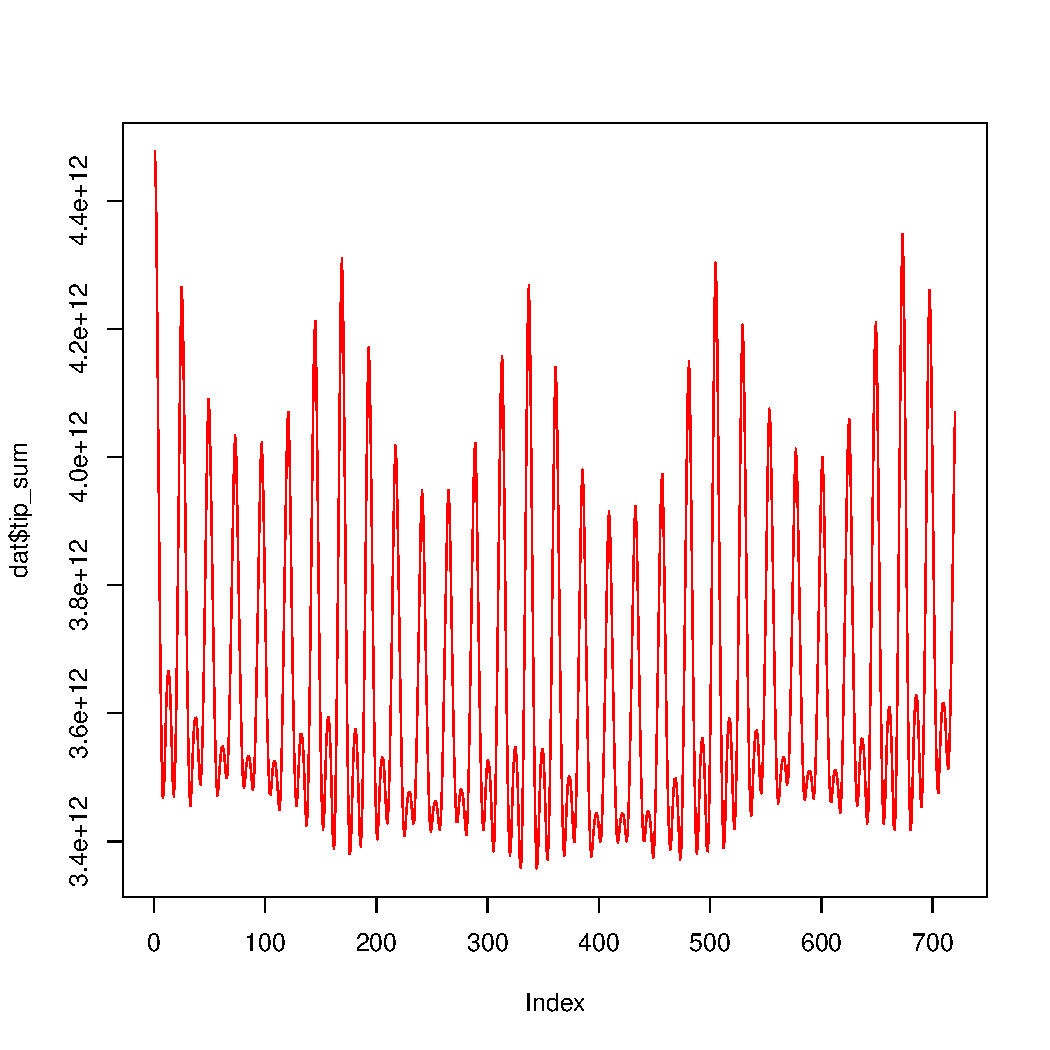
\includegraphics[page=1,scale=0.35]{plot/autocorr}
    }
    \subfigure[Autocorrelation of hourly trip count]{
      \label{fig:tipcountautocorr}
      \includegraphics[page=2,scale=0.35]{plot/autocorr}
    }

    \subfigure[Autocorrelation of hourly tip average]{
      \label{fig:tipavgautocorr}
      \includegraphics[page=3,scale=0.35]{plot/autocorr}
    }
  \end{figure}

  The plots indicate that evening to midnight was the busiest hour, especially in weekends. Drivers could receive more tip mostly because there were more business. The average tip amountm, however, did not show clear seasonality. 

  \subsection{K-nearest-neighbor Tip Predictor}
  One of the simplest learning algorithm is call K-nearest-neighbor. The algorithm predicts unknown values by comparing the input with known instances. The algorithm requires large amount of data and computing power. However, it suits well on Hadoop. In our implementation of the algorithm, we first calculated the distance between the input and each record, then Top-K pattern was employed to efficiently choose the K nearest neighbors. To predict a numerical value, we needed to calculate the average of the K values. Because K was normally a small value, we used a python script to programmatically retrieve the top K values and calculate the average. The command-line application takes into account pickup, dropoff Lat-lon coordination, vender, day of week, hour of day, and rate code (type of trip).



  \section{Performance}
  Our execution environment was on a cluster of at least 36 nodes. All the nodes were virtual machines on a 2.4GHz 8-core Intel Xeon E5530. Each job spawned 36 mappers, one or up to 24 reducers, according to the computation need. The Hadoop block size was configured as 128MB. However, we used a unsplittable compression format (gzip). Thus each mapper read a whole file, or about 180MB. Because of a bug (described in Section \ref{sec:assortedsummary}), each input file was read nearly twice. 
  The observed performance of is illustrated below (see Table \ref{tab:performance}).
  \begin{table}[h]
    \center
    \caption{Performance}
    \label{tab:performance}
    \begin{tabular}{|c|c|}\hline
      Job & execution time\\  \hline
      Numerical Summary & 1:12\\  \hline
      Factor Summary & 1:48\\  \hline
      Correlation & 1:40\\  \hline
      $\chi^2$ & 1:58\\  \hline
      Autocorrelation & 2:40\\  \hline
      KNN & 5:12\\  \hline
    \end{tabular}
  \end{table}

  \section{Discussion}
  The results clearly indicates that tipping behaviors are highly influenced by temporal, spacial and psychological factors. However, the results are not comprehensive. As is true of any statistical investigation, the results are limited in terms of causality. For example, the valleys in hourly pick up count may be caused not by the demand for taxi services, but by congested traffic conditions.

  Future analysis of the data set can split the data into more granular pieces and use ANOVA test to determine the dependence between  categorical variables and numerical variables. To better understand tipping behavior, researches can focus on categorizing different tipping patterns based on regions, time, venders and etc.

  The KNN predictor should only be used as a guidance. The model has not been validated thoroughly. Based on our manual validation, the predictor can sometimes give noisy results, because the learning data set has only gone through basic outlier removal only and KNN in particular is not resistive to noisy data. Besides, the KNN predictor performed badly in regions with sparse data.

  Future implementation of the data set can first add weighting factors based on distances or regional norms. Further, a to achieve more understanding of tipping behaviors and more precise prediction, one can use the regression tree algorithm.

  We hope that this article cast light on high performance statistical calculations with Hadoop.
  \cleardoublepage
  \phantomsection
  \addcontentsline{toc}{section}{References}
  \printbibliography 
  \end{document}

